\section{Introduction}
\label{sec:intro}

% Abstractive summarization 

%Abstractive summarization is designed for generating a fluent and concise summary output covering key points given the source input. 
%Prior studies mainly focus on datasets with monologue inputs such as news including CNN/DM\cite{hermann2015teaching} and XSum\cite{narayan2018don}, and scientific publications including PubMed\cite{cohan2018discourse}. 

% dialogue summarization task
Recently, dialogue summarization has attracted increasing attention due to its necessity and usefulness. The inputs for this task are utterances generated from multiple participants in the first person, including scenarios such as online written chat-logs, daily spoken dialogues, meeting transcripts, etc. 
It generates fluent and concise summaries in a third-person point of view as shown in Figure \ref{fig:example}, helping people to go through the main ideas of a dialogue for quickly joining the conversation or reminding of conclusions or agreements.  
Different from previous monologue inputs such as news~\cite{narayan2018don} and scientific publications~\cite{cohan2018discourse}, dialogues are always less well-organized. They usually contain complicated reference relations, inconsecutive inter-utterance dependencies, informal expressions, and so on, making dialogue summarization a more challenging task.



 \begin{figure}
	\centering
	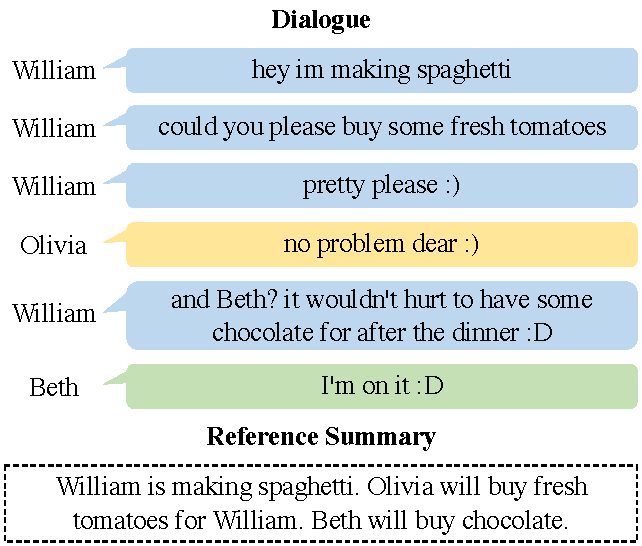
\includegraphics[scale=0.63]{example.pdf}
	\caption{An example from SAMSum dataset. Different colors for utterances is used to identify different speakers.}
	\label{fig:example}
\end{figure}
%\begin{table}
%	\centering
%	\small
%	
%	\begin{tabular}{|p{1.2cm}p{6.3cm}|}
%		\hline
%		\multicolumn{2}{|c|}{\textbf{Dialogue}} \\
%		\hline
%		William& hey im making spaghetti \\
%		William& could you please buy some fresh tomatoes \\
%		William& pretty please :) \\
%		Olivia& no problem dear :) \\
%		William& and Beth? it wouldn't hurt to have some chocolate for after the dinner :D \\		
%		Beth& I'm on it :D\\
%		\hline
%		\multicolumn{2}{|c|}{\textbf{Reference Summary}} \\
%		\hline
%		\multicolumn{2}{|p{7.8cm}|}{William is making spaghetti. Olivia will buy fresh tomatoes for William. Beth will buy chocolate.}\\
		%BART&Olivia will buy some fresh tomatoes for the spaghetti. Beth will buy chocolate for after the dinner.\\
		%Multi-view&William is making spaghetti. Olivia will buy fresh tomatoes and chocolate for after the dinner.\\
		%DialoGPT&William is making spaghetti . Olivia will buy some fresh tomatoes and some chocolate for after the dinner .\\
		%Dial2Text&William is making spaghetti. Olivia will buy fresh tomatoes and Beth will buy chocolate for after the dinner.\\		
%		\hline
%	\end{tabular}
	
%	\caption{A sample of the original dialogue and its summary from SAMSum dataset.}\label{tab:example}  
%\end{table}

% previous work:
%Remarkable works on news summarization, such as RNN-based models including Pointer-Generator~\cite{see2017get} and Fast-Abs-RL~\cite{chen2018fast} , and transformer-based models including pretrained BART~\cite{lewis2020bart}, can be directly applied to dialogue summarization tasks by concatenating all of the utterances sequentially as the source input. However, such concatenation operation largely overlooks dialogue features, such as structure information inter and intra utterances, and results in unsatisfied dialogue summaries. 

% \begin{figure*}
%	\centering
%	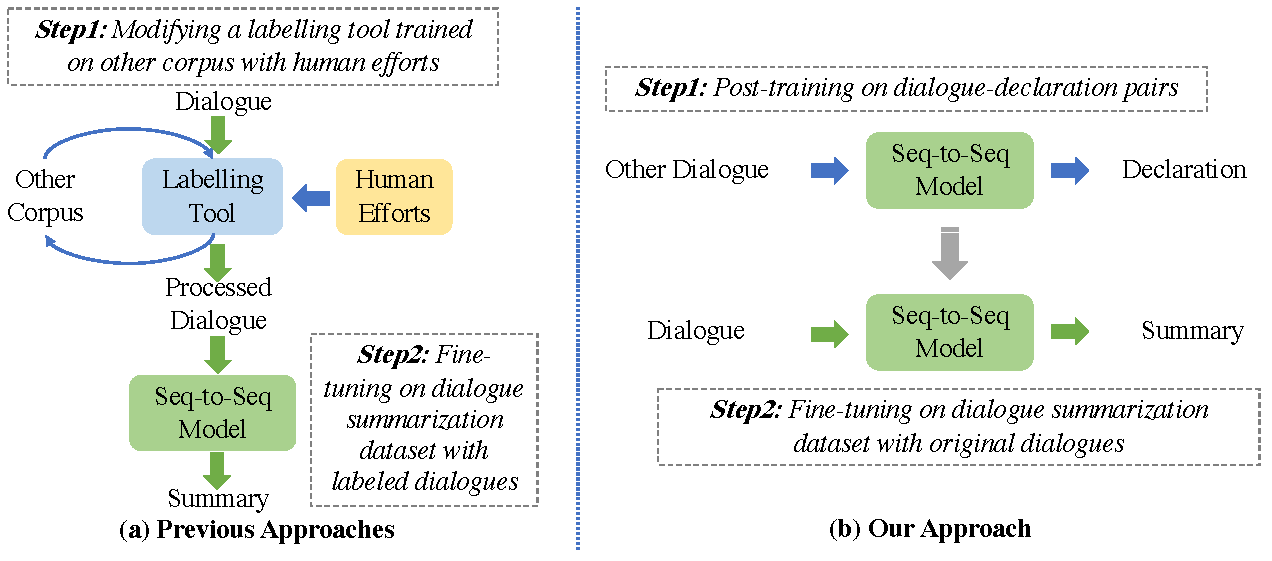
\includegraphics[scale=0.65]{model.pdf}
%	\caption{Comparison of previous methods and our approach.}
%	\label{fig:approach}
%\end{figure*}




% pretrain models
The most intuitive characteristic of dialogue summarization is the different 
text formats between its dialogue and summary. As mentioned in Liu, Shi and Chen's work~\shortcite{liu2021coreference}, coreference resolution models trained on general narrative text get around 10\% lower performance on dialogue corpus, demonstrating the inherent gap between dialogue and narrative text.
However, pretrained language models nowadays are barely trained on a single text format. For example, DialoGPT~\cite{zhang2020dialogpt} and PLATO~\cite{bao2020plato} are trained on dialogue corpus for dialogue generation or selection tasks, and BART~\cite{lewis2020bart} and PEGASUS~\cite{zhang2020pegasus} are trained on general text corpus for translation or news summarization tasks. So, they are not ideal for such cross-format tasks.



Considering the format divergence, we can naturally regard the dialogue summarization task into two complementary learning subtasks:
1) rephrasing from dialogue to narrative text; 2) selection of contents to be summarized. 
Previous models are trained to learn these two subtasks simultaneously.
They focus on injecting dialogue features into pretrained language models such by data preprocessing on dialogues % with small modifications to the model 
as shown in Figure \ref{fig:approach1}. 
Some features are more relevant to the rephrasing ability, such as coreference relations~\cite{liu2021coreference}, discourse graphs and action graphs~\cite{chen2021structure}. The other features, such as stage segmentation, topic segmentation~\cite{chen2020multi} and redundancy detection~\cite{feng2021language}, tend to emphasize on content selection. This also supports the idea of regarding dialogue summarization into two subtasks.


However, these previous works suffer from two weaknesses. 
First, these data labeling approaches are transferred from their original designed domains and need human labors to design different hyper-parameters or rules for adapting to different dialogue summarization datasets, such as the
%weights between two views in Multi-view~\cite{chen2020multi} and 
rules in~\citet{liu2021coreference}.
Second, above mentioned features may not generalize well to different dialogue scenarios. For example, the argument graph~\cite{fabbri2021convosumm} for capturing key argumentative contents is not suitable for e-mail threads as mentioned in their paper. %and for daily dialogues as shown in Figure \ref{fig:example}.



% our solution
In this work, we learn these two subtasks one by one.
%\footnote{We don't cut the whole task into isolated sub-tasks, and just put more effort on each task during different training stages.}.
Firstly, we propose to do post-training with cross-format data, i.e., further train the pre-trained language model towards rephrasing from dialogue to narrative text.
%We propose doing cross-format post-training for dialogue summarization towards learning to rephrase from dialogue to general text as the first step.
%\KZ{I suggest not use the word ``cross-format''. It's not about format, more about 
%styles. Format sounds more mechanical. Style sounds more natural. Also, people might be
%wondering what's the difference between ``rephrasing'' into a declaration and ``summarizating'' into a summary.}
%We hypothesize that pre-training between different formats can help capture cross-format information and results in better dialogue summarization performances.
% dataset
Due to the lack of paired cross-format data covering the same contents and participants, we collect more than 30k dialogue-declaration pairs by transforming the question-answering pairs from dialogue reading comprehension datasets into their declaration form. Since each declaration usually talks about parts of a dialogue, we introduce a prefix-guided generation task to help the model focus on learning to express specified information according to the dialogue in a third-person point of view.
%we take advantage of the widely accepted dialogue reading comprehension(RC) datasets such as DREAM~\cite{sun2019dream} and  FriendsQA~\cite{yang2019friendsqa}. By transform the question-answering pairs into their declaration form, we collect more than 30k dialogue-declaration training pairs for cross-format pre-training.
% pretrain task
%Since each dialogue may be paired with multiple declarations and each declaration is only about part of the dialogue, we propose a pre-training task with prefix-guided generation strategy both during training and inferencing to guide the model focus on learning to express dialogue-related information in a third-person point of view.
Then, we further finetune the post-trained model on dialogue summarization datasets, concentrating on learning the content selection ability.
\begin{figure}[t]
	\centering
	\subfigure[Previous Approaches]{
		%		\centering
		%		\begin{minipage}[t]{0.5\linewidth}
		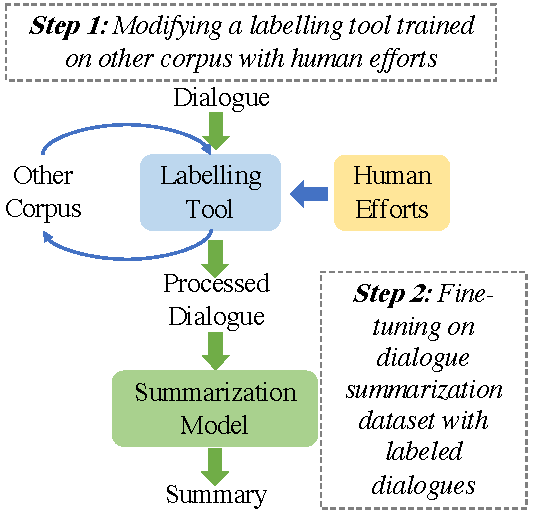
\includegraphics[scale=0.6]{model-1.pdf}\label{fig:approach1}
		%		\end{minipage}
	}
	
	\subfigure[Our Approach]{
		%	\centering
		%	\begin{minipage}[t]{0.5\linewidth}
		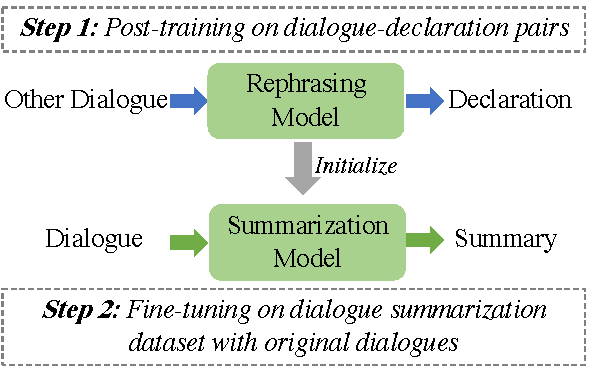
\includegraphics[scale=0.6]{model-2.pdf}\label{fig:approach2}
		%	\end{minipage}
	}
	\caption{Illustrations of previous approaches and our approach. Blue arrows refers to processes only used for training, and greens ones for both training and inference.}
	\label{fig:approach}
\end{figure}

%experiment
%We do post-training on the pretrained language model BART. 
%For downstream applications, 
A number of datasets for dialogue summarization tasks %cross different scenarios and granularities 
are covered, including online written dialogue dataset SAMSUM~\cite{gliwa2019samsum}, daily spoken dialogue dataset DialSumm~\cite{chen2021dialsumm}, email thread dataset Email~\cite{fabbri2021convosumm} and high-level topic description dataset TopicAMI~\cite{goo2018abstractive}. 
% solve the previous weaknesses % more strength
With our post-training approach, laboured work on data preprocessing and feature engineering for each application scenario is no longer needed. 
Experiments show the favorable results of our model over strong baselines and the state-of-the-art models.

%We also do few-shot experiments on SAMSUM datasets, and the results prove that our approach is more robust and gets better performance in such low data resource settings. 

% our contributions
In a word, our contributions are:
\begin{itemize}
\item As far as we know, we are the first to train models to learn the rephrasing ability on cross-format datasets. We will release the new cross-format dataset for further research (Sec \ref{sec:dcd}) and experiments demonstrate that we successfully narrow the comprehension gap of neural models between dialogues and narrative texts(Sec \ref{sec:ablations}).
 
\item We propose to regard the dialogue summarization into two complementary subtasks and we are the first to do post-training for this task with the cross-format dataset and propose a prefix-guided generation task(Sec \ref{sec:pgt}). %\&\ref{sec:dpdresults}
Our approach significantly outperforms BART and achieving competitive results with the state-of-the-art methods on the well-known SAMSum corpus(Sec \ref{sec:automaticevaluation}).

%\KZ{This is hardly a contribution.}
% for better understanding of the relationship between a dialogue and its declarations.
%And the generalization ability cross dialogue scenarios and summarization granularities are proved according to the comprehensive experiments.
\item Comprehensive experiments on dialogue summarization tasks across different dialogue scenarios and levels of summarization granularity demonstrate the strong generalization ability of our approach(Sec \ref{sec:automaticevaluation}\&\ref{sec:humaneval}).
% \KZ{Focus on this part and make some meaningful
%conclusion from our experiments.}
\end{itemize}




